\tikzset{
    vertex/.style = {
        circle,
        fill            = black,
        outer sep = 2pt,
        inner sep = 1pt,
    }
}
\begin{figure}[H]
    \centering
    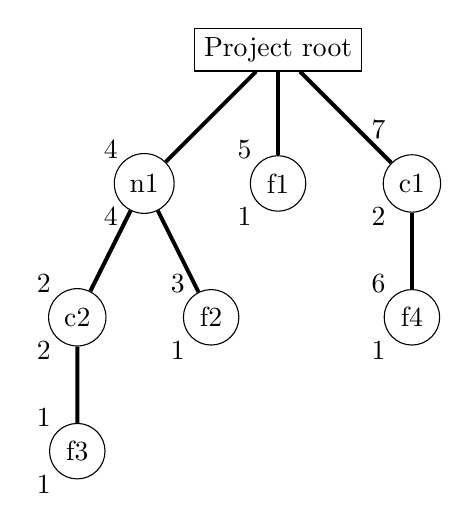
\begin{tikzpicture}[scale=0.85]
        % root
        %\node at (0.0, 1.0) {Project root};
        \node[draw] (root) at (0.0, 0.0) {Project root};
        
        %root scope
        %\node at (4, 1.0) {level 1}; 
        \node[draw, circle] (n1) at (-2, -2) {n1};       \draw[line width=0.5mm,draw=black] (root) to (n1);
        \node at (-2.5, -2.5) {4};    \node at (-2.5, -1.5) {4};
            \node[draw, circle] (c2) at (-3.0, -4.0) {c2};   \draw[line width=0.5mm,draw=black] (n1) to (c2);
            \node at (-3.5, -4.5) {2};    \node at (-3.5, -3.5) {2};
                \node[draw, circle] (f3) at (-3.0, -6.0) {f3};   \draw[line width=0.5mm,draw=black] (c2) to (f3);
                \node at (-3.5, -6.5) {1};    \node at (-3.5, -5.5) {1};
            \node[draw, circle] (f2) at (-1.0, -4.0) {f2};   \draw[line width=0.5mm,draw=black] (n1) to (f2);
            \node at (-1.5, -4.5) {1};    \node at (-1.5, -3.5) {3};
        \node[draw, circle] (f1) at (0, -2.0) {f1};    \draw[line width=0.5mm,draw=black] (root) to (f1);
        \node at (-0.5, -2.5) {1};    \node at (-0.5, -1.5) {5};
        \node[draw, circle] (c1) at (2, -2.0) {c1};     \draw[line width=0.5mm,draw=black] (root) to (c1);
        \node at (1.5, -2.5) {2};    \node at (1.5, -1.2) {7};
            \node[draw, circle] (f4) at (2.0, -4.0) {f4};   \draw[line width=0.5mm,draw=black] (c1) to (f4);
            \node at (1.5, -4.5) {1};    \node at (1.5, -3.5) {6};
        
        
    \end{tikzpicture}
    \caption{Local to global index example.}
    \label{fig:treeIndex}
    \medskip
    \small
    Figure \ref{fig:treeIndex} shows a project with one namespace, one class and one function in global-scope, one class in the namespace and one function in each class. Top number is global-index and lower number is local-index.
\end{figure}